\subsection{Mise à jour}
\vspace{1cm}

Toutes les informations récupérées et calculées jusqu’à maintenant, devaient pouvoir être mises à jour régulièrement via un script simple. J’ai donc mis en place un composant spécialement dédiée à cette action, qui lance de façon procédurale la mise en place de la base de données et la récupération complète de tous les éléments précédemment introduits.

Cette classe prend en paramètre des identifiants fédéraux valides, nécessaires au lancement des méthodes CURL, ainsi qu’une clé API Google active.

\begin{figure}[!h]
    \centering
    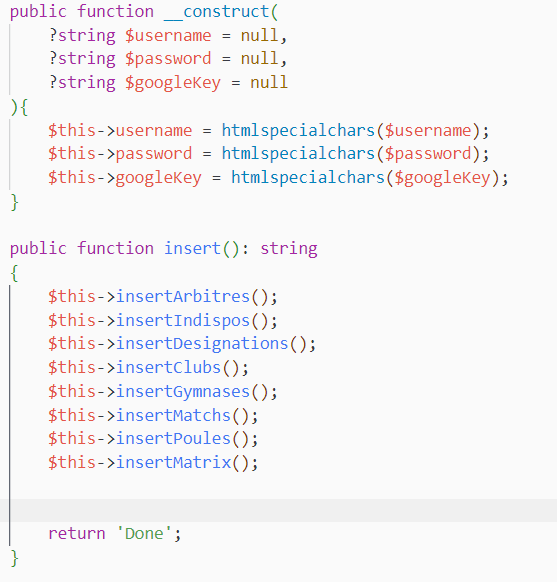
\includegraphics{update_code.png}
    \caption{Méthode principale du composant de mise à jour de la BDD}
\end{figure}

Un appel à la méthode \colored{insert()} de cette classe crée la base de données définie dans le fichier de configuration \colored{globals.php} (voir configuration), en prenant en compte le nom des tables et colonnes définies dans le fichier \colored{config.json}, puis insère toutes les données nécessaires au projet depuis les différentes classes de celui-ci.